\documentclass[modern]{aastex61}

%% Reintroduced the \received and \accepted commands from AASTeX v5.2
%\received{July 1, 2016}
%\revised{September 27, 2016}
\draft{\today}
%% Command to document which AAS Journal the manuscript was submitted to.
%% Adds "Submitted to " the arguement.
\submitjournal{ApJ}

%% Mark up commands to limit the number of authors on the front page.
%% Note that in AASTeX v6.1 a \collaboration call (see below) counts as
%% an author in this case.
%
%\AuthorCollaborationLimit=3
%

\shorttitle{\aastex\ Astropy Project II}
\shortauthors{Astropy Project et al.}

\begin{document}

\title{Astropy - New software standards for a growing community}

%%
%% The \author command is the same as before except it now takes an optional
%% arguement which is the 16 digit ORCID. The syntax is:
%% \author[xxxx-xxxx-xxxx-xxxx]{Author Name}
%%
%% This will hyperlink the author name to the author's ORCID page. Note that
%% during compilation, LaTeX will do some limited checking of the format of
%% the ID to make sure it is valid.
%%
%%
%% The new \altaffiliation can be used to indicate some secondary information
%% such as fellowships. This command produces a non-numeric footnote that is
%% set away from the numeric \affiliation footnotes.  NOTE that if an
%% \altaffiliation command is used it must come BEFORE the \affiliation call,
%% right after the \author command, in order to place the footnotes in
%% the proper location.
%%
%% Use \email to set provide email addresses. Each \email will appear on its
%% own line so you can put multiple email address in one \email call. A new
%% \correspondingauthor command is available in V6.1 to identify the
%% corresponding author of the manuscript. It is the author's responsibility
%% to make sure this name is also in the author list.
%%
%% While authors can be grouped inside the same \author and \affiliation
%% commands it is better to have a single author for each. This allows for
%% one to exploit all the new benefits and should make book-keeping easier.
%%
%% If done correctly the peer review system will be able to
%% automatically put the author and affiliation information from the manuscript
%% and save the corresponding author the trouble of entering it by hand.

\correspondingauthor{Astropy Coordinating committee or First Author}
\email{coordinators@astropy.org}

\author{Astropy Project}

\begin{abstract}

Astropy is amazing. and even more amazing than before

\end{abstract}

%% Keywords should appear after the \end{abstract} command. 
%% See the online documentation for the full list of available subject
%% keywords and the rules for their use.
\keywords{}

\section{Introduction} \label{sec:intro}

Moritz volunteered to write the intro


Deciding if a feature should be included
difficulty to decide where general use ends and "handy feature for some" starts, i.e. how to reject PRs or deal with maintenance burden

\section{Major concepts}
\subsection{Astropy development model, astropy ecosystem}
This subsection should include some basic statistics about the contributors, commits, line of code etc. up to the 2.0 release when we know it.
\subsection{Mixin}
\subsection{Accuracy testing across many different implementation}

%\subsection{Difficulty of reversing design choices}
\section{Key features}

The astropy project aims to provide python-based packages for all tasks that are commonly needed in a large subset of the astronomical community. Two aspects of this (time and coordinate transformations) are already discussed in great detail in section 3. In this section, we highlight other features introduced or substantially improved since version v0.2, which is described in Astropy Collaboration et al. (2013).
(ordered in the order in which they appear in the astropy documentation)

\subsection{Constants}
versioning 

\subsection{Coordinates}



start with short description of the astropy approach and features (JPL ephemerids, barycentric correction, proper motions, coordinate frames) then shows the tests. In particular, we had a discussion on problems with the definition of some coordinate system on the mailing list. Getting that discussion in here gives us a refereed paper to point to when we need to push the IAU to fix that.

\subsection{Units and quantities}

incl logarithmic units and magnitudes
speed improvements,
interaction with numpy arrays

\subsection{Data arrays}

\subsubsection{NDDdata}

\subsubsection{Tables}
QTable is new, mixin columns for time and coordinates. Table operations were added in v0.3

\subsection{Convolution}
Astropy implements `normalized convolution' (e.g., Knutsson and Westin 1993; http://ieeexplore.ieee.org/abstract/document/341081/), which is an image reconstruction technique in which missing data are ignored during the convolution and replaced with values interpolated using the kernel.   In version $<=1.3$, the direct convolution and fft convolution approaches were not consistent, with fft convolution implementing normalized convolution and direct convolution implementing a different approach.  As of v2.0, the two methods are consistent and include a suite of consistency checks.


\begin{figure}
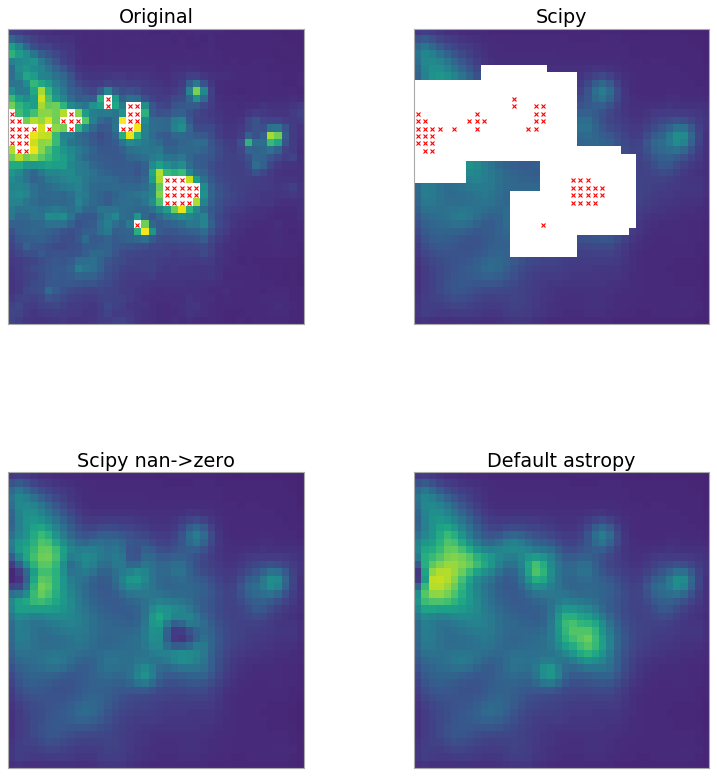
\includegraphics[width=\textwidth]{convolution_example.png}
An example showing different modes of convolution available in the python ecosystem.  The red x's mark pixels that are set to NaN in the original data (a).  If the data are convolved with a Gaussian kernel on a 9x9 grid using scipy's direct convolution (b), any pixel within range of the original NaN pixels is also set to NaN.  Panel (c) shows what happens if the NaNs are set to zero first: the originally NaN regions are depressed relative to their surroundings.  Finally, panel (d) shows astropy's convolution behavior, where the missing pixels are replaced with values interpolated from their surroundings using the convolution kernel.
\end{figure}


\subsection{Modeling}
The whole modeling submodule was missing from the previous paper, so everything really, including compound models, unit support etc.

\subsection{Visualization}
wcsaxis, rgb, histograms comes to mind.Can use more publicity and also makes good images to include in the paper.

\subsection{Statistics}
%Crawford and JV


major additions to be discussed: lomb-scargle, sigma clipping, bayesian blocks, histograms

\section{Infrastructure for affiliated packages}
\subsubsection{Package template}
\subsection{Continuous integration helpers}
bsipocz should write this up
\subsection{sphinx extensions}
probably Tom R should write this up
\section{State of the Ecosystem}

\section{Tutorials, Snippets, Gallery}

\section{Outlook}
dropping python2 support, growths of affiliated packages
Summary

\acknowledgments

Who to thank?

%% Similar to \facility{}, there is the optional \software command to allow 
%% authors a place to specify which programs were used during the creation of 
%% the manusscript. Authors should list each code and include either a
%% citation or url to the code inside ()s when available.

\software{astropy \citep{2013A&A...558A..33A},  
          numpy, 
          scipy, 
          }
          
%\bibliographystyle{aasjournal}          
%\bibliography{bibliography}

\begin{thebibliography}{}

\end{thebibliography}



\end{document}

